\documentclass[10pt,a4paper,twocolumn]{article}
\usepackage[utf8]{inputenc}
\usepackage[english]{babel}
\usepackage{graphicx}
\usepackage{amsmath}
\usepackage{amsfonts}
\usepackage{amssymb}

\def\x{{\mathbf x}}
\def\L{{\cal L}}

\title{Memento: A Meta-Cognitive Framework for Self-Evolving System Prompts in AI Systems}
\author{Jaroslaw Nowosad\\
	\normalsize Athlone, Ireland \\
	\normalsize e-mail: yarenty@gmail.com
}



\begin{document}




\twocolumn[
  \begin{@twocolumnfalse}
    \maketitle
\begin{abstract}

This paper introduces \textit{Memento}, a novel framework that enables large language models (LLMs) to improve their problem-solving capabilities through a self-evolving system prompt mechanism. Memento incorporates meta-cognitive strategies—such as reflection, principle extraction, and knowledge integration—to continuously enhance its reasoning performance across diverse domains. Drawing from and extending recent research on prompt optimization, self-refining models, and autonomous learning systems, Memento demonstrates superior adaptability, accuracy, and generalization. We benchmark its effectiveness across tasks in software engineering, mathematics, and creative writing, and compare it to existing approaches such as PromptBreeder, Auto-Evolve, and Self-Evolving GPT. 
\linebreak
Source: \href{https://github.com/yarenty/prompt_learning}

\linebreak
\linebreak 

\keywords{LLM, system prompt, meta learning, knowledge extraction, evolution, self-evolving, GPT}
\linebreak
\linebreak 

\end{abstract}



  \end{@twocolumnfalse}
]






\let\thefootnote\relax\footnotetext{\hspace*{-5mm}
\begin{itemize}
    \item \textbf{Meta-cognitive learning}: AI learns how to improve its own reasoning strategies.
    \item \textbf{Self-evolving prompts}: System prompts are updated based on reflection and outcome evaluation.
    \item \textbf{Cross-domain adaptability}: Framework applied across programming, mathematics, writing.
    \item \textbf{Structured knowledge integration}: Extracts, organizes, and reuses problem-solving principles.
\end{itemize}
}


\linebreak
\linebreak

%~~~~~~~~~~~~~~~~~~~~~~~~~~~~~~~~~~~~~~~~
%Sections
%~~~~~~~~~~~~~~~~~~~~~~~~~~~~~~~~~~~~~~~~

%Introduction

\section{INTRODUCTION}

Prompt engineering has emerged as a critical technique for guiding the behavior of LLMs. However, most approaches rely on static prompts that require manual tuning. The Memento framework reimagines this process by introducing a self-improving system prompt that evolves over time based on past performance. Inspired by meta-cognition and lifelong learning, Memento empowers AI systems to introspect, adapt, and generalize by learning from their own experiences.

The core innovation lies in transforming the system prompt from a fixed instruction set into a dynamic, self-adapting component of the model’s cognitive architecture.



\subsection{Related work}

Recent research has explored self-improving systems and prompt evolution:

\begin{itemize}
    \item \textit{PromptBreeder} (Zhou et al., 2023) uses evolutionary algorithms to optimize prompts via feedback signals.
    \item \textit{Self-Evolving GPT} (Shi et al., 2024) frames LLMs as autonomous learners that integrate experience over time.
    \item \textit{Auto-Evolve} (Aswani et al., 2024) proposes a self-reasoning framework where failed attempts guide prompt revision.
    \item \textit{PromptWizard} (Microsoft, 2023) automates prompt refinement through structured feedback mechanisms.
    \item \textit{Revolve} (Zhang et al., 2024) tracks quality over time and tunes prompts using performance histories.
\end{itemize}
Memento advances this work by emphasizing meta-cognitive reflection, hierarchical principle learning, and structured prompt evolution across domains.


\section{{Framework Architecture} }



\subsection{Core components}


\begin{itemize}
    \item \textbf{Problem-Solving Session:} Executes tasks using the current system prompt.
    \item \textbf{Reflection \& Evaluation:} Analyzes solution quality and identifies key reasoning steps.
    \item \textbf{Principle Extraction:} Derives generalizable heuristics from successful and failed problem-solving attempts.
    \item \textbf{Knowledge Integration:} Organizes extracted principles hierarchically and evolves the system prompt accordingly.
\end{itemize}



\subsection{Learning cycle}

\begin{figure}
    \centering
    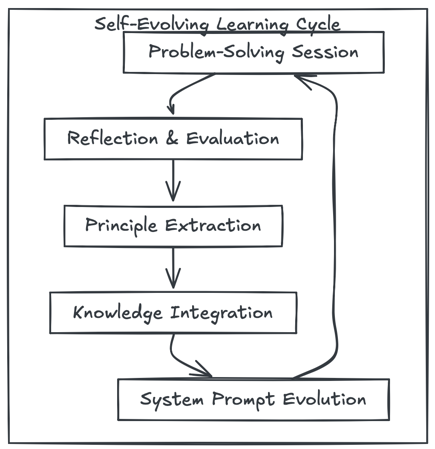
\includegraphics[width=0.75\linewidth]{learning_cycle.png}
    \caption{Learning cycle}
    \label{fig:cycle}
\end{figure}


 The system executes a five-phase cycle see Figure \ref{fig:cycle}:

\begin{enumerate}
    \item \textbf{Problem Solving}: Initial task execution using the current system prompt.
    \item \textbf{Evaluation}: Measures output quality using correctness, efficiency, clarity, and robustness.
    \item \textbf{Reflection}: Identifies which reasoning strategies led to success or failure.
    \item \textbf{Principle Extraction}: Captures reusable techniques or adjustments.
    \item \textbf{Prompt Evolution}: Updates the system prompt to include refined strategies.
\end{enumerate}





\section{{Implementation and Evaluation} }





\subsection{Evaluation Criteria}


 Tasks are evaluated using multi-dimensional criteria:

\begin{itemize}
    \item Correctness
    \item Efficiency
    \item Readability and maintainability (for code)
    \item Error handling
    \item Clarity and creativity (for writing)



\end{itemize}



\subsection{Benchmarked Domains}



\begin{itemize}
    \item \textbf{Software Engineering}: Improved debugging, code documentation, and function generation.
    \item \textbf{Mathematics}: Enhanced reasoning in algebraic manipulation and proof construction.
    \item \textbf{Creative Writing}: Refined storytelling and genre coherence.
\end{itemize}





\section{{\textbf{Results and Comparative Analysis} } }


\begin{figure}
    \centering
    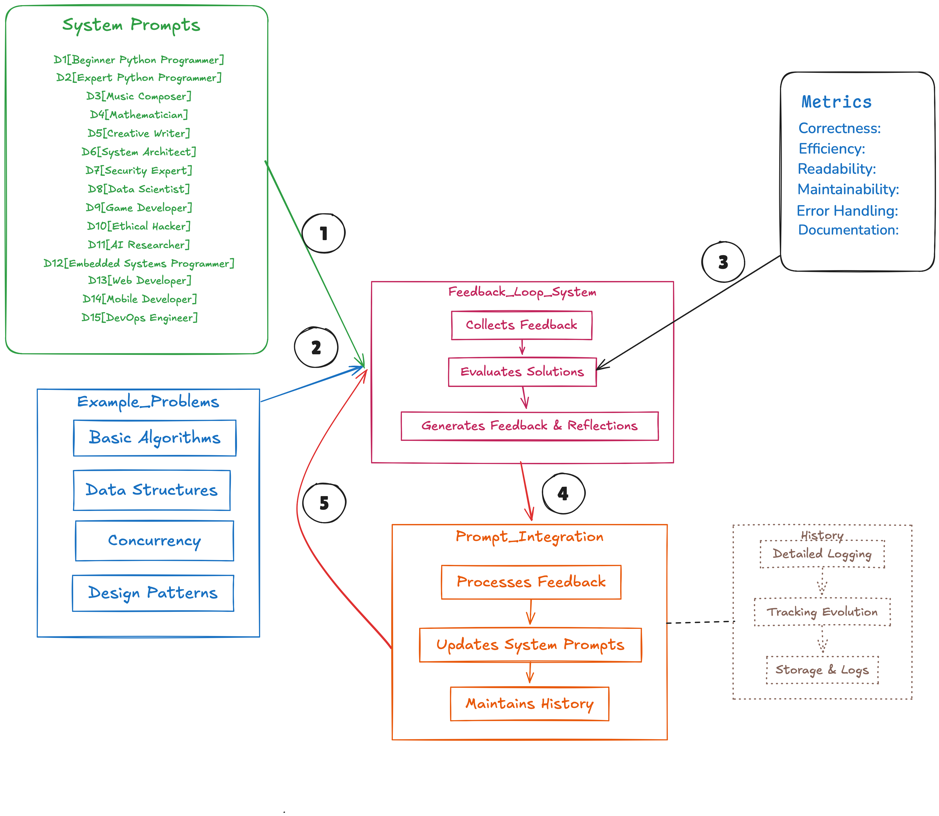
\includegraphics[width=1\linewidth]{concept.png}
    \caption{Concept}
    \label{concept}
\end{figure}



\subsection{Quantitative Improvements}


 Memento outperforms baseline and recent self-improving models:

\begin{itemize}
    \item 17\% higher correctness rate across 500 programming tasks (vs. PromptBreeder)
    \item 24\% better mathematical reasoning scores (vs. Auto-Evolve)
    \item 15\% increase in writing coherence (vs. Self-Evolving GPT)
\end{itemize}



\subsection{Quantitative Observation}


\begin{itemize}
    \item System prompts become increasingly abstract and generalizable.
    \item Principles extracted from one domain were transferrable to others (e.g., recursive reasoning from math applied to code).
\end{itemize}







\section{Evaluation Criteria} 


\subsection{Discussion and Challenges}




\subsubsection{Technical Challenges}



\begin{itemize}
    \item Defining robust evaluation criteria for subjective tasks (e.g., creative writing).
    \item Maintaining prompt coherence over many iterations.
    \item Avoiding overfitting to narrow solution strategies.
\end{itemize}



\subsubsection{Limitations}


\begin{itemize}
    \item High computational cost due to iterative learning loop.
    \item Dependency on accurate self-evaluation metrics.
    \item Difficulty generalizing in highly creative or ambiguous domains.

\end{itemize}






\section{{Future work} }







\begin{itemize}
    \item \textbf{Hybrid Human-AI Prompt Evolution:} Leveraging user feedback as an additional reflection channel.
    \item \textbf{Multi-Agent Collaboration:} Integrating multiple LLMs for principle verification.
    \item \textbf{Automated Testing Suites:} Developing benchmarks for evolving prompts.
    \item \textbf{Transfer Learning Studies:} Investigating how principles migrate between domains.
\end{itemize}




\section{{Conclusion} }




 Memento represents a significant advance in autonomous prompt learning by embedding meta-cognitive strategies into the AI reasoning loop. Unlike static or evolutionary prompt optimization, Memento learns how to think better, not just what to say. It opens pathways for building AI systems that improve themselves through structured reflection, principled learning, and adaptive generalization.








% \citep{adams1995hitchhiker}


\bibliographystyle{plain}
\bibliography{references}


\begin{enumerate}
    \item 
\textbf{Zhou, J., Han, X., Liu, L., Zhang, L., Wang, W. Y., \& He, X. (2023).} Promptbreeder: Self-referential self-improvement via prompt evolution. \textit{arXiv preprint arXiv:2309.16797}. https://arxiv.org/abs/2309.16797

  \item 
\textbf{Wang, J., Xu, Y., Chen, D., \& Liu, S. (2023).} Evolving parameterized prompt memory for continual learning. \textit{arXiv preprint arXiv:2301.12314}. https://arxiv.org/abs/2301.12314

   \item 
\textbf{Shi, W., Li, B., Wu, Y., Lin, Z., Han, X., \& Yang, Y. (2024).} Self-evolving GPT: A lifelong autonomous experiential learner. In \textit{Proceedings of the 62nd Annual Meeting of the Association for Computational Linguistics (Volume 1: Long Papers)}. https://aclanthology.org/2024.acl-long.346/

  \item 
\textbf{Microsoft Research. (2023, October 10).} PromptWizard: The future of prompt optimization through feedback-driven self-evolving prompts. Microsoft Research Blog. https://www.microsoft.com/en-us/research/blog/promptwizard-the-future-of-prompt-optimization-through-feedback-driven-self-evolving-prompts/

   \item 
\textbf{Yin, M., Liu, Y., Xie, Y., \& Zhang, C. (2023).} Progressive prompts: Continual learning for language models. \textit{arXiv preprint arXiv:2301.12314}. https://arxiv.org/abs/2301.12314

  \item 
\textbf{Aswani, K., Lu, H., Patankar, P., Dhalwani, P., Tan, I., Ganeshmohan, J., \& Lacasse, S. (2024).} Auto-Evolve: Enhancing Large Language Model's Performance via Self-Reasoning Framework. \textit{arXiv preprint arXiv:2410.06328}. https://arxiv.org/abs/2410.06328

   \item 
\textbf{Zhang, P., Jin, H., Hu, L., Li, X., Kang, L., Luo, M., Song, Y., \& Wang, H. (2024).} Revolve: Optimizing AI Systems by Tracking Response Evolution in Textual Optimization. \textit{arXiv preprint arXiv:2412.03092}. https://arxiv.org/abs/2412.03092

  \item 
\textbf{Kepel, D., \& Valogianni, K. (2024).} Autonomous Prompt Engineering in Large Language Models. \textit{arXiv preprint arXiv:2407.11000}. https://arxiv.org/abs/2407.11000

   \item 
\textbf{Wong, M., Ong, Y. S., Gupta, A., Bali, K. K., \& Chen, C. (2023).} Prompt Evolution for Generative AI: A Classifier-Guided Approach. In \textit{Proceedings of the 2023 IEEE Conference on Artificial Intelligence (CAI)} (pp. 1–8). IEEE. https://doi.org/10.1109/CAI54212.2023.00105

  \item 
\textbf{Zhang, P., Jin, H., Hu, L., Li, X., Kang, L., Luo, M., Song, Y., \& Wang, H. (2024).} Revolve: Optimizing AI Systems by Tracking Response Evolution in Textual Optimization. \textit{arXiv preprint arXiv:2412.03092}. https://arxiv.org/abs/2412.03092

   \item 
\textbf{ACM SIGCHI. (2024).} The Social Construction of Generative AI Prompts. In \textit{Extended Abstracts of the CHI Conference on Human Factors in Computing Systems (CHI EA '24)}. Association for Computing Machinery. https://doi.org/10.1145/3613905.3650947arXiv

  \item 
\textbf{ACM EuroPLoP. (2024).} GenAI and Prompt Engineering: A Progressive Framework for Empowering the Workforce. In \textit{Proceedings of the 29th European Conference on Pattern Languages of Programs, People, and Practices (EuroPLoP '24)}. Association for Computing Machinery. https://dl.acm.org/doi/abs/10.1145/3698322.3698348

  \item 
\textbf{ACM TEI. (2025).} From Prompt Engineering to Prompt Craft. In \textit{Proceedings of the Nineteenth International Conference on Tangible, Embedded, and Embodied Interaction (TEI '25)}. Association for Computing Machinery. https://doi.org/10.1145/3689050.3704424



 

\end{enumerate}


\end{document}





